%\vspace{-4mm}

\section{Introduction}
\label{sxn:intro}

XXX.  INTRO

\charlesX{in the Intro, we need to build directly off Hidary and Poggios work}
Figure~\ref{fig:vgg_lognorms} plots $\langle\log\Vert\mathbf{W}\Vert_{F}\rangle$ vs the reported (Top1) test accuracy for the series of pre-trained VGG models (available in the pyTorch package~\cite{pyTorch}). 

Notice we did not need to peek at the test data to make this plot.  
In fact, we did not need the ImageNet training data either.  
Amazingly, the average log norm is well correlated with the reported test accuracies.

\begin{figure}[!htb]
 \centering
   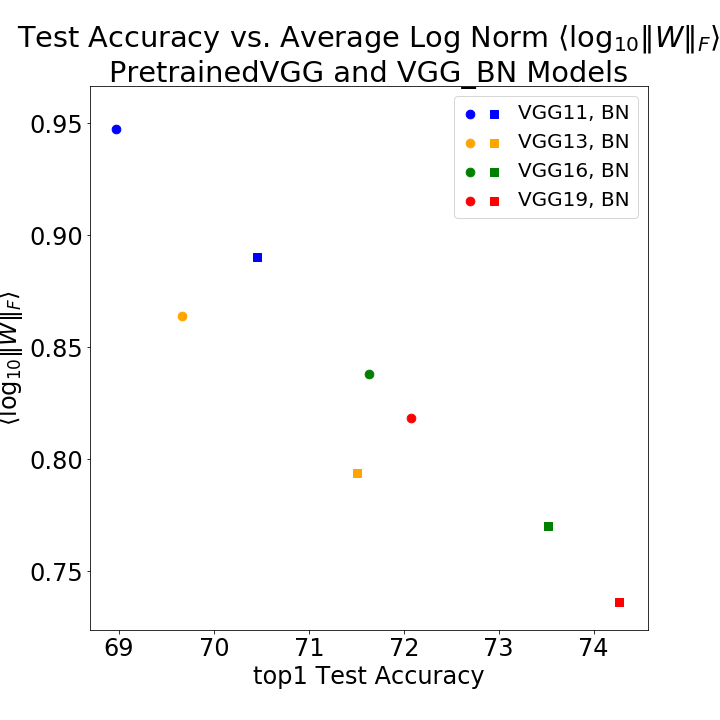
\includegraphics[scale=0.40]{img/vgg-lognorms.png}
   \caption{
Pretrained VGG and VGG BN Architectures and DNNs.  Test Accuracy and average log Frobenius norm $\langle\log\Vert\mathbf{W}\Vert_{F}\rangle$ for
 VGG11 vs VGG11\_BN ({\color{blue}{blue}}),
VGG13 vs VGG13\_BN ({\color{orange}{orange}}),
VGG16 vs VGG16\_BN ({\color{green}{green}}),  and
VGG19 vs VGG19\_BN ({\color{red}{red}}). 
}
  \label{fig:vgg_lognorms}
\end{figure}

We believe this is the first time this theoretical complexity metric has been reported to predict (trends in) the test accuracy for production
DNNs.  This in itself is remarkable.  But we can do even better than this -- by exploiting Heavy Tail Universality.


Next, see Figure \ref{fig:vgg_alphahat} for our improvements, using the method we introduce below.

\begin{figure}[!htb]
 \centering
   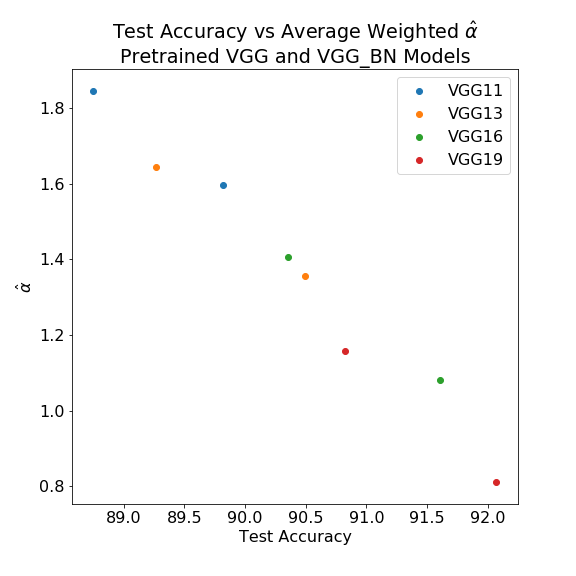
\includegraphics[scale=0.40]{img/vgg-w_alphas.png}
   \caption{
Pretrained VGG and VGG BN Architectures and DNNs.  Test Accuracy and weighted average $\hat{\alpha}$ for
 VGG11 vs VGG11\_BN ({\color{blue}{blue}}),
VGG13 vs VGG13\_BN ({\color{orange}{orange}}),
VGG16 vs VGG16\_BN ({\color{green}{green}}),  and
VGG19 vs VGG19\_BN ({\color{red}{red}}). 
}
  \label{fig:vgg_alphahat}
\end{figure}

In summary, our main results are the following:
\begin{itemize}
\item
We apply the product norm regularization metric to the VGG series of models, illusrtating that it performs moderately well.
\item
We use HT-RMT and the recently-developed theory of implicit self-regularization to develop a novel capacity metric.
\charlesX{THIS:  We use our recently-developed Theory of Heavy Tailed Self-Regularization (HT-SR) to develop a novel capacity metric}
This metric is a linear combination of PL exponents, where the coefficients are the spectral norm of something; and this metric may be viewed as a refinement of the product norm metric to account for finite-size effects.
\item
We apply this novel metric to the VGG series, showing that it does better than the product norm metric; and we apply it to a wide range of other pre-trained models, including XXX, XXX, and XXX.
\charlesX{THIS: We apply our nee metric to all the available pretrained DNNs, including the VGG series, the numerous ResNet architectures, and numerous other popular models. It generally does as well or better than the  product norm metric}

\end{itemize}

